\documentclass[a4paper,12pt]{article}
\usepackage{sbc-template}
\usepackage[utf8]{inputenc}
\usepackage{graphicx}
\usepackage{amsmath,amsthm,amsfonts,amssymb}
\usepackage[mathcal]{eucal}
\usepackage{latexsym}
\usepackage[brazil]{babel}
\usepackage{bm}
\usepackage[all]{xy}
\usepackage{indentfirst}
\usepackage{fancyhdr}
\usepackage[portuguese, ruled, linesnumbered]{algorithm2e}
\usepackage{subfigure}
\usepackage[pdftex]{hyperref}
\usepackage{float}
\sloppy

\title{Comparação entre algoritmos sequencial e paralelo utilizados na resolução de multiplicação entre matrizes\\}

\author{Taylan Branco Meurer\inst{1}, Leandro Loffi\inst{1}, Rodrigo Curvello\inst{2}}


\address{Acadêmico Ciência da Computação -- Instituto Federal Catarinense -- Campus Rio do Sul
          (IFC)\\
          %Caixa Postal 15.064 -- 91.501-970 -- Porto Alegre -- RS -- Brazil
        \nextinstitute
          Professor Ciência da Computação -- Instituto Federal Catarinense -- Campus Rio do Sul\\
          \email{tbmeurer@gmail.com, leandroloffi3@gmail.com,
          rodrigo.curvello@ifc-riodosul.edu.br}
        }


\begin{document} 

\maketitle

\begin{abstract}
This paper compares the performance of serial and parallel algorithms . The algorithms perform a multiplication of square matrices and will be written in C , Java and Python. Parallelism was performed by OpenMP library, Jomp , the multiprocessing and Cython language. The runtimes were obtained by the time command from a bash terminal. The metric used is based on Amdahl Act, so the language with better performance in parallel has the largest speedup . The algorithms were run on a machine with Intel Core I7-3630QM with SSD ( mSATA ) and Debian stretch Operating System and Gnome 3.20. 
\end{abstract}

\begin{resumo}
Neste trabalho compara-se o desempenho de algoritmos seriais e paralelos. Os algoritmos realizam uma multiplicação entre matrizes quadradas e serão escritos em C, Java e Python. O paralelismo foi efetuado através da biblioteca OpenMP, do Jomp, do Multiprocessing e da linguagem Cython. Os tempos de execução foram obtidos por meio do comando time de um terminal bash. A métrica utilizada é baseada na Lei de Amdahl, portanto a linguagem com melhor desempenho em paralelo tem o maior speedup. Os algoritmos foram executados em uma máquina com Intel Core I7-3630QM, com SSD (mSATA) e com Sistema Operacional Debian stretch e Gnome 3.20.
\end{resumo}
\section{Introdução}

O trabalho trata sobre serialização e paralelismo de algoritmos. Os algoritmos em série são aqueles executados linha após linha por um único processador e algoritmos paralelos são aqueles executados por dois ou mais processadores ao mesmo tempo. 

	As linguagens de programação paralela surgiram como um novo recurso para facilitar a tarefa de construir programas que utilizem os recursos de paralelismo de equipamentos com arquitetura de computação paralela \cite{sato}. Para utilizar plenamente os recursos de um equipamento multiprocessado, existem basicamente duas opções, construir programas com controle sobre os trechos de paralelismo, utilizando recursos de uma Linguagem de Programação para a criação das threads e processos necessários, ou utilizar-se de uma biblioteca, a qual, normalmente, é composta por diretivas de compilador para uma linguagem de programação pré-existente, como C.
	 
	Desde a criação dessas arquiteturas, surgiram diversas bibliotecas ou APIs, entre elas a OpenMP, que será utilizada nesse trabalho. O desenvolvimento  desta API foi realizado através de um trabalho colaborativo entre os diversos parceiros interessados no projeto, entre eles: Compaq/Digital, Hewlett-Packard, Intel, IBM, KAI, Silicon Graphics, Sun entre outros \cite{sato}. 
	
	O trabalho busca analisar e comparar o desempenho entre as linguagens Java, Python e C para execução de um algoritmo de multiplicação entre matrizes. As matrizes serão quadradas e terão ordem 500, 1500 e 2000. O desempenho será avaliado com emprego da lei de Amdahl e com o comando time do shell GNU/Linux em bash. 
	
	Conforme Albuquerque\footnote{ALBUQUERQUE, Jones. {\bf Lei de Amdahl.}. Recife: DFM-UFRPE: 2004} (2004), a lei de amdahl é uma maneira de expressar o speedup máximo como uma função da quantidade de paralelismo e da fração da computação que é inerentemente sequencial. O speedup máximo $(S)$ alcançado por um computador paralelo com $p$ processadores executando a computação é:
	
\begin{equation}
  \label{eq:amdahl}
   S \le \frac{1}{f + \frac{(1-f)}{p}}
\end{equation}

A linguagem C fará uso da API OpenMP, a Java do Jomp e a Python do  OpenMP com Cython.

O trabalho irá no capítulo seguinte tratar sobre a API OpenMP e a linguagem Cython. Em seguida, abordará a metodologia empregada para a construção do trabalho. Posteriormente, apresentará os resultados e, por último, relatará as considerações finais e as referências bibliográficas. 

\section{Processamento Paralelo}
Processamento paralelo consiste na divisão de uma determinada tarefa em tarefas menores e na execução de cada uma dessas tarefas em diferentes processadores \cite{tutopenmp}. Conforme \cite{william}, existem dois conceitos de paralelismo: de instruções e de máquina. O paralelismo de instruções existe quando as instruções de uma sequência são independentes e o de máquina é definido como uma medida da capacidade do processador em aproveitar o paralelismo no nível de instruções.

O processamento paralelo pode acontecer em ambientes de memória distribuída ou compartilhada. Segundo \cite{tutopenmp}, processamento paralelo em memória distribuída consiste na distribuição de tarefas para serem executadas em diferentes processadores com recursos próprios de memória. Processamento paralelo em ambientes de memória compartilhada consiste na divisão das tarefas entre vários processadores que compartilham o mesmo recurso de memória global.

Nesse capítulo será apresentado de forma genérica informações sobre OpenMP, Multiprocessing e Cython. 
\subsection{OpenMP}

A API OpenMP oferece um conjunto de diretivas para a programação paralela em sistemas multiprocessados com memória compartilhada, realizando para tal a criação e o controle de Threads \cite{sato}. As diretivas da OpenMP podem ser incluídas em programas escritos nas linguagens “C” e FORTRAN para especificar pedaços de programas que devem ser executados em paralelo.

O Open specification for Multiprocessing, simplesmente OpenMP, é um modelo de programação em memória compartilhada, que faz uso da especificação Pthreads. Ele surgiu a partir da cooperação de grandes fabricantes, como: Sun, IBM, Intel, AMD, HP, etc. Projetada para operar em C e Fortran, as especificações são diretivas que dizem ao compilador como gerar códigos paralelos. 


\begin{figure}[!htb]
  \centering
  \caption{Paralelismo.}
  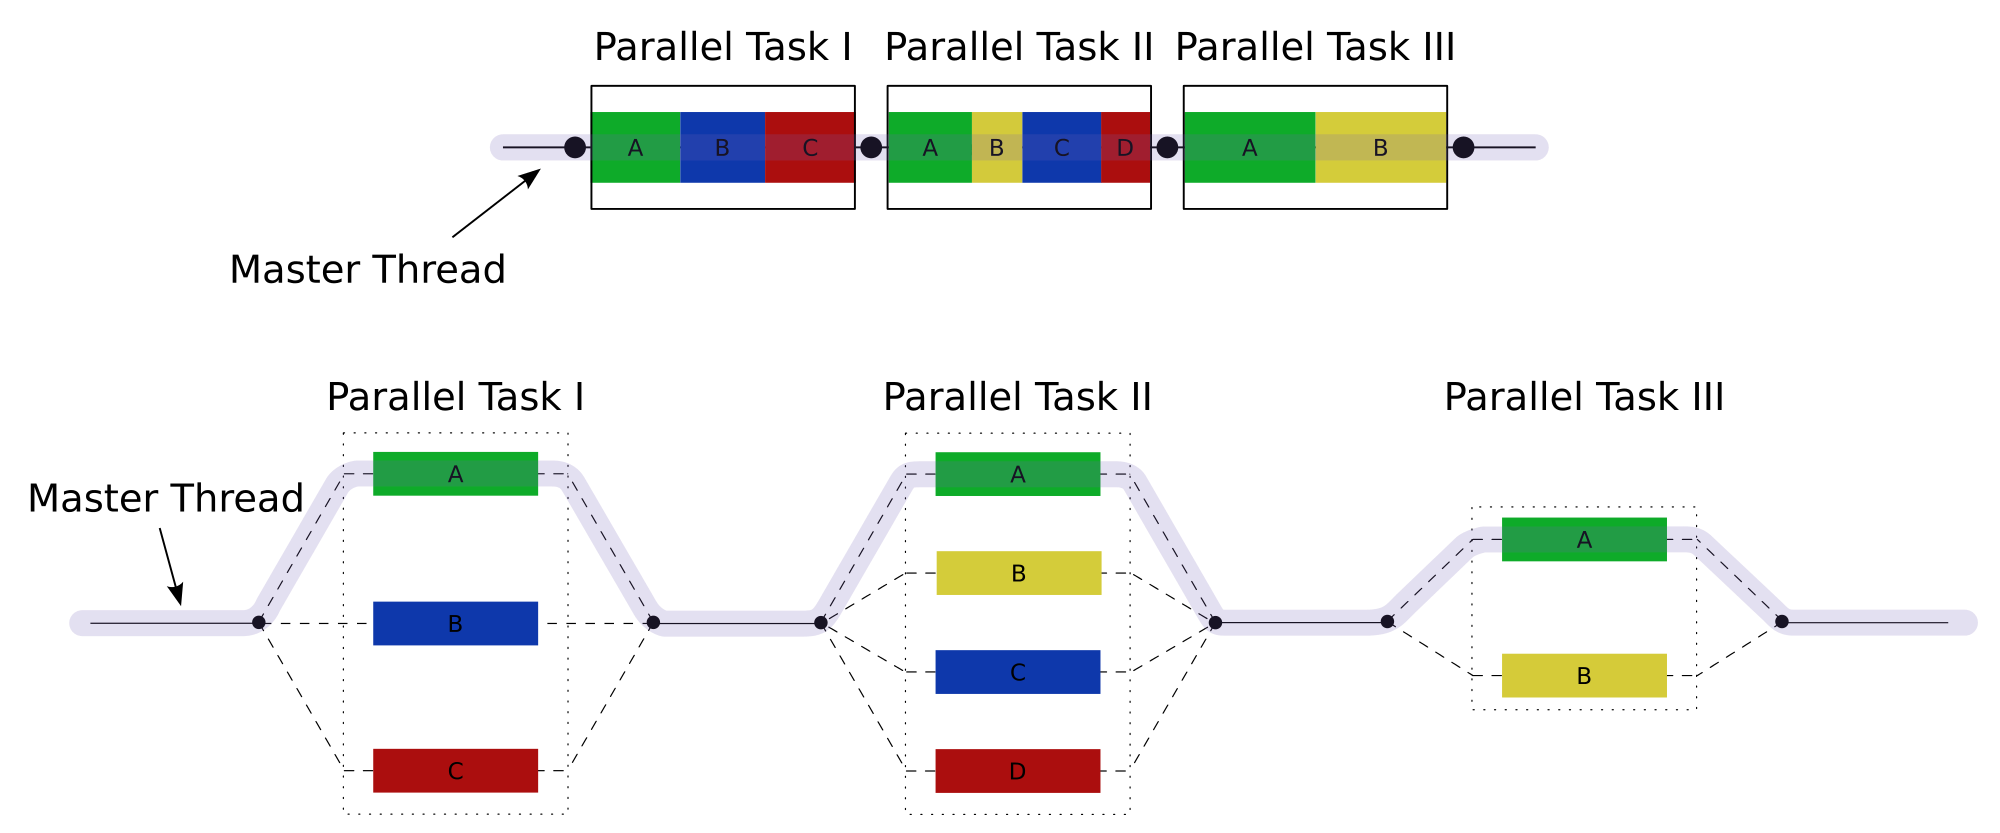
\includegraphics[width=15cm]{pictures/parallel.png}
  \footnotesize{Fonte: OpenMP\footnotemark}
\label{fig:parallel}
\end{figure}
\footnotetext{Disponível em:$<$https://upload.wikimedia.org/wikipedia/commons/thumb/f/f1/Fork\underline{\hspace{0.1cm}}join.svg/2000px-Fork\underline{\hspace{0.1cm}}join.svg.png$>$ Acessado em: 05 de julho de 2016.}

Conforme a figura \ref{fig:parallel}, pode-se visualizar a forma como pode ser realizado a divisão e como funciona um programa com tarefas paralelas. A primeira tarefa é executada por 3 núcleos, a segunda tarefa em 4 núcleos e, por último, a terceira tarefa foi dividida para ser executada em paralelo por 2 núcleos. Entre as tarefas, existe uma área comum serial, a qual pode representar um local de memória compartilhada. 

Internamente a OpenMP trabalha com um modelo “FORK-JOIN” onde a partir de uma
“thread master” (aquela que iniciou o programa) cria-se um time de threads para a
realização de tarefas em paralelo, e depois é realizado um join onde todas as threads
são sincronizadas e destruídas, sobrando somente a master thread.

O algoritmo 1 demonstra um exemplo básico do uso de uma instrução em paralelo com OpenMP. A partir do algoritmo é possível verificar o emprego das diretivas e dos parâmetros da API. Na linha 2, verifica-se a diretiva do construtor paralelo, o mais importante do OpenMP, uma vez que é o responsável pela indicação da região do código que será executado em paralelo \cite{tutopenmp}. Ainda na linha 2, estão inclusas três cláusulas do construtor, a saber, shared, private e num\underline{\hspace{0.1cm}}threads. O shared diz respeito às variáveis que são compartilhadas, o private recebe como parâmetros as variáveis privadas e o num\underline{\hspace{0.1cm}}threads recebe o número de threads que serão utilizadas para execução paralela. Na linha 4 e 12, emprega-se o construtor for, que faz com que as iterações da estrutura de repetição situada logo abaixo da diretiva sejam executadas em paralelo \cite{tutopenmp}.    


A próxima seção irá contemplar breves informações sobre o módulo de paralelismo para Python - multiprocessing e Cython. 

\subsection{Multiprocessing}
Multiprocessing\footnote{Disponível em:$<$https://docs.python.org/2/library/multiprocessing.html$>$ Acessado em: 23 de junho de 2016.} é um módulo Python para processamento paralelo. Ele faz uso de uma API semelhante ao threading. 
O pacote multiprocessing oferece concorrência local e remota, contornando o Global Interpreter Lock através de subprocessos no lugar de threads. Por essa razão, esse módulo permite ao programador tirar proveito total dos múltiplos processadores em uma determinada máquina.
O multiprocessing também apresenta APIs com características distintas do módulo threading. Um bom exemplo disso é o objeto Pool, o qual oferece um meio conveniente de paralelização por meio de uma função com vários valores de entrada, distribuindo esses dados de entrada nos processos (paralelismo de dados). 

\subsection{Cython}
Cython é um compilador estático otimizado para Python \cite{cython}. A linguagem Cython\footnote{Disponível em:$<$http://cython.org/$>$ Acessado em: 05 de julho de 2016} é um superconjunto da linguagem Python que suporta chamar funções e declarar tipos de dados C. Isso permite ao compilador gerar códigos em C eficientes a partir de um código Cython. Quase todo código em Python é válido em Cython. 

Com o emprego do Cython, garante-se, no mínimo, 25\% de ganhos com relação ao Python puro. A virtude do Cython é a sua capacidade de usar variáveis e parâmetros como tipos de dados em C. As variáveis e parâmetros podem ser misturadas sem afetar a execução \cite{cython}. Além disso, o Cython suporta paralelismo nativo através do módulo {\bf cython.parallel}, que emprega a API OpenMP. 

\section{Algoritmo}
A seguir será demonstrado o pseudocódigo do algoritmo utilizado no trabalho para execução paralela em C. Para obter o serial basta remover as diretivas do openmp: \#pragma omp argumento. 

\begin{algorithm}[!htb]
   \SetAlgoLined   
   \Entrada{Definir variáveis (i,j,k) e a constante SIZE\\
            Inicializar as matrizes (A,B,C) de ordem SIZE\\
            Definir número de threads (NUM)\\
           }
   \Inicio
   { 
       \#pragma omp parallel shared(A,B,C) private(i,j,k) num\underline{\space}threads(NUM) \\
       \{\\
        \#pragma omp for\\
        \Para{cada i até SIZE}
        {
            \Para{cada j até SIZE}
            {
                $A[i][j] = 3 \ast  i +  j$\\
        				$B[i][j] = i +  3 \ast  j$\\
	    	    		$C[i][j] = 0$\\
            }  
            
            
        }
        
        \#pragma omp for\\
        \Para{cada i até SIZE}
        {
            \Para{cada k até SIZE}
            {
                \Para{cada j até SIZE}
                {
                   $C[i][j] = C[i][j] + A[i][k] \ast  B[k][j]$\\
                }
            }
        }
      \}
    
   }
   \label{alg:MxM}
   \caption{algoritmo paralelo}
\end{algorithm}


\section{Metodologia}
A metodologia faz uso da linguagem C, Java e Python (versão 2.7). Cada linguagem é composta por dois algoritmos, um serial e outro paralelo. O código paralelo em C é implementado com uso da API OpenMP. Em Java, o paralelismo é feito com Jomp e em Python com multiprocessing e Cython. 

O algoritmo implementa uma multiplicação entre matrizes. Essa implementação é bastante conhecida e generalista. Além disso, exige grande esforço computacional. Os tempos de execução foram obtidos por meio do comando de terminal {\it time}\footnote{Disponível em: $<$http://ss64.com/bash/time.html$>$ Acessado em: 22 de junho de 2016.}. Este comando registra o tempo de CPU utilizado e retorna o valor em segundos.  

Os testes foram executados em uma máquina Intel Core I7 3630QM\footnote{Disponível em:$<$http://ark.intel.com/pt-br/products/71459/Intel-Core-i7-3630QM-Processor-6M-Cache-up-to-3\underline{\hspace{0.1cm}}40-GHz$>$ Acessado em: 20 de junho de 2016.}, CPU 3.4 GHz, 6MB de cache. A máquina possui 8GB de memória RAM e faz uso de um SSD mSATA. O Sistema Operacional instalado é o Debian stretch com kernel 4.6.0-1-amd64 e Gnome.

\section{Resultados e discussões}

Os resultados foram atingidos por meio do comando time para o terminal em bash. Um exemplo de execução é demonstrado a seguir: 
$\$\hspace{0.1cm} time \hspace{0.1cm} python \hspace{0.1cm}programa.py$

O comando time retorna o tempo de execução do programa em segundos. A definição do tempo de execução se deu conforme a equação \ref{eq:tempo_exec}.

\begin{equation}
  \label{eq:tempo_exec}
   T_{medio} = \frac{T_{1} + T_{2} + T_{3}}{3}
\end{equation}

Uma vez descoberto os tempos de execução, o próximo cálculo realizado foi o do speedup. Este demonstra o ganho de desempenho obtido com a paralelização. A equação \hyperlink{eq:amdahl}{\ref{eq:amdahl}} demonstra como se deu o procedimento de obtenção do speedup.

Os tempos de execução e os speedups calculados serão demonstrados a seguir por meio de tabelas e gráficos. 

\begin{table}[H]
  \centering
  \caption{Tempo de execução -- C}
  \begin{tabular}{ccc}
    \hline
    Matriz(ordem) & Serial(s) & Paralelo(s)\\
    \hline
    \hline
    500 & 0.446 & 0.127\\
    1000 & 3.292 & 0.898\\
    1500 & 11.461 & 3.189\\
    2000 & 26.847 & 7.235\\
    \hline
  \end{tabular}
  \label{tab:timec}
\end{table}


%\begin{figure}[!htb]
%  \centering
%  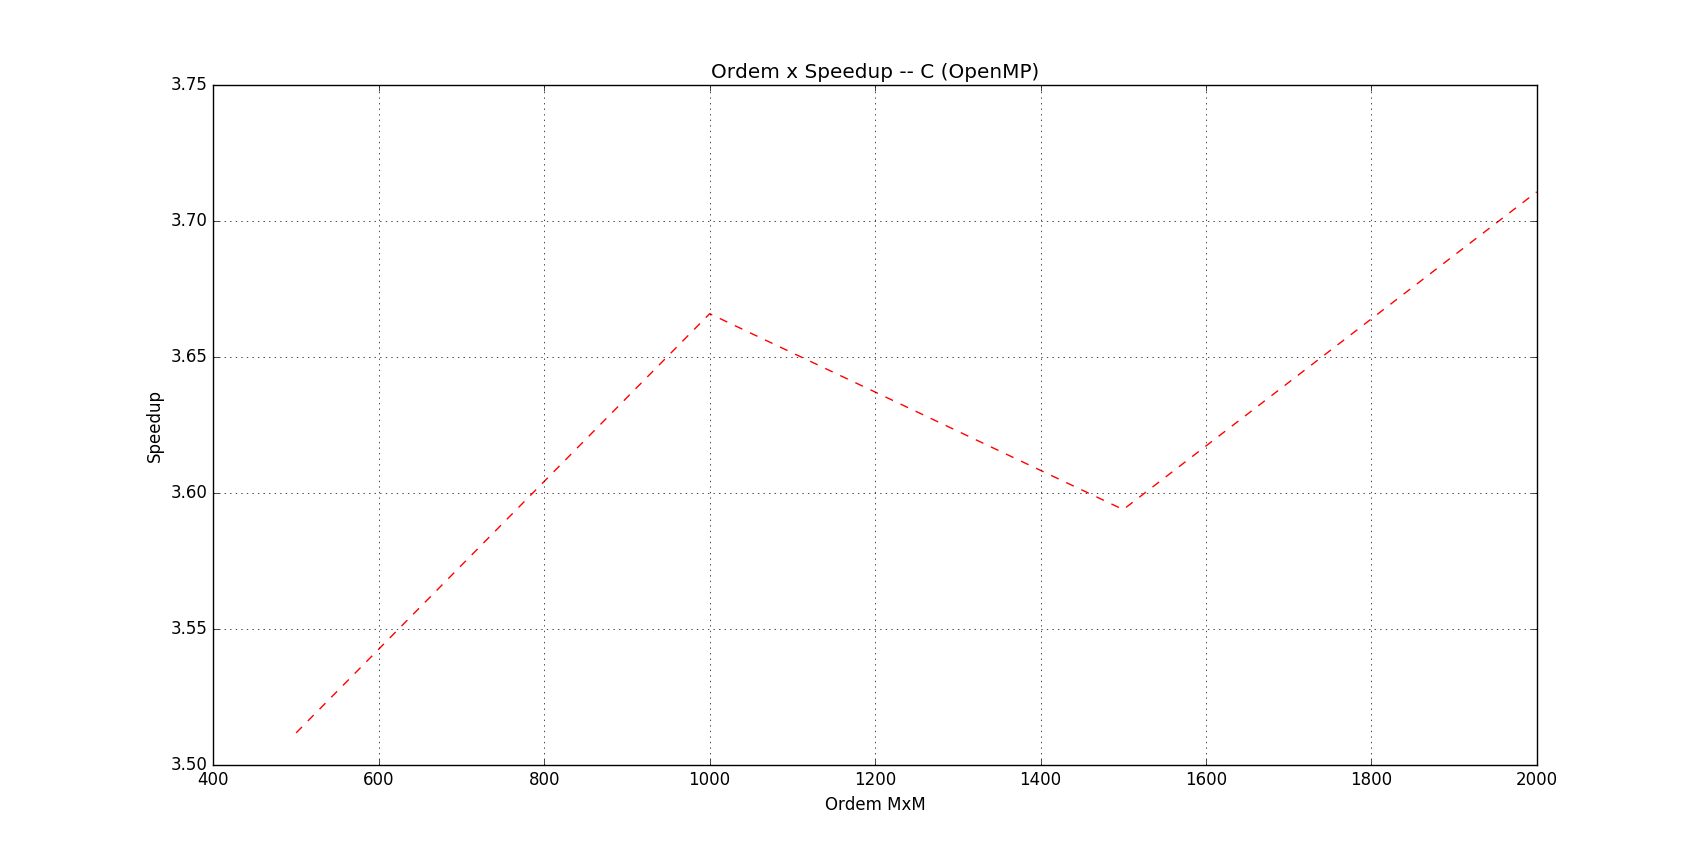
\includegraphics[width=15.0cm]{pictures/speedup_C.png}
%  \caption{Ordem x Speedup - C (OpenMP)}
%\label{fig:speedup_C}
%\end{figure}


\begin{table}[H]
  \centering
  \caption{Tempo de execução -- Java}
  \begin{tabular}{ccc}
    \hline
    Matriz(ordem) & Serial(s) & Paralelo(s) -- Jomp\\
    \hline
    \hline
    500 & 0.228 & 0.189\\
    1000 & 0.845 & 0.413\\
    1500 & 2.590 & 1.000\\
    2000 & 6.274 & 2.157\\
    \hline
  \end{tabular}
  \label{tab:timeJava}
\end{table}

%\begin{figure}[!htb]
%  \centering
%  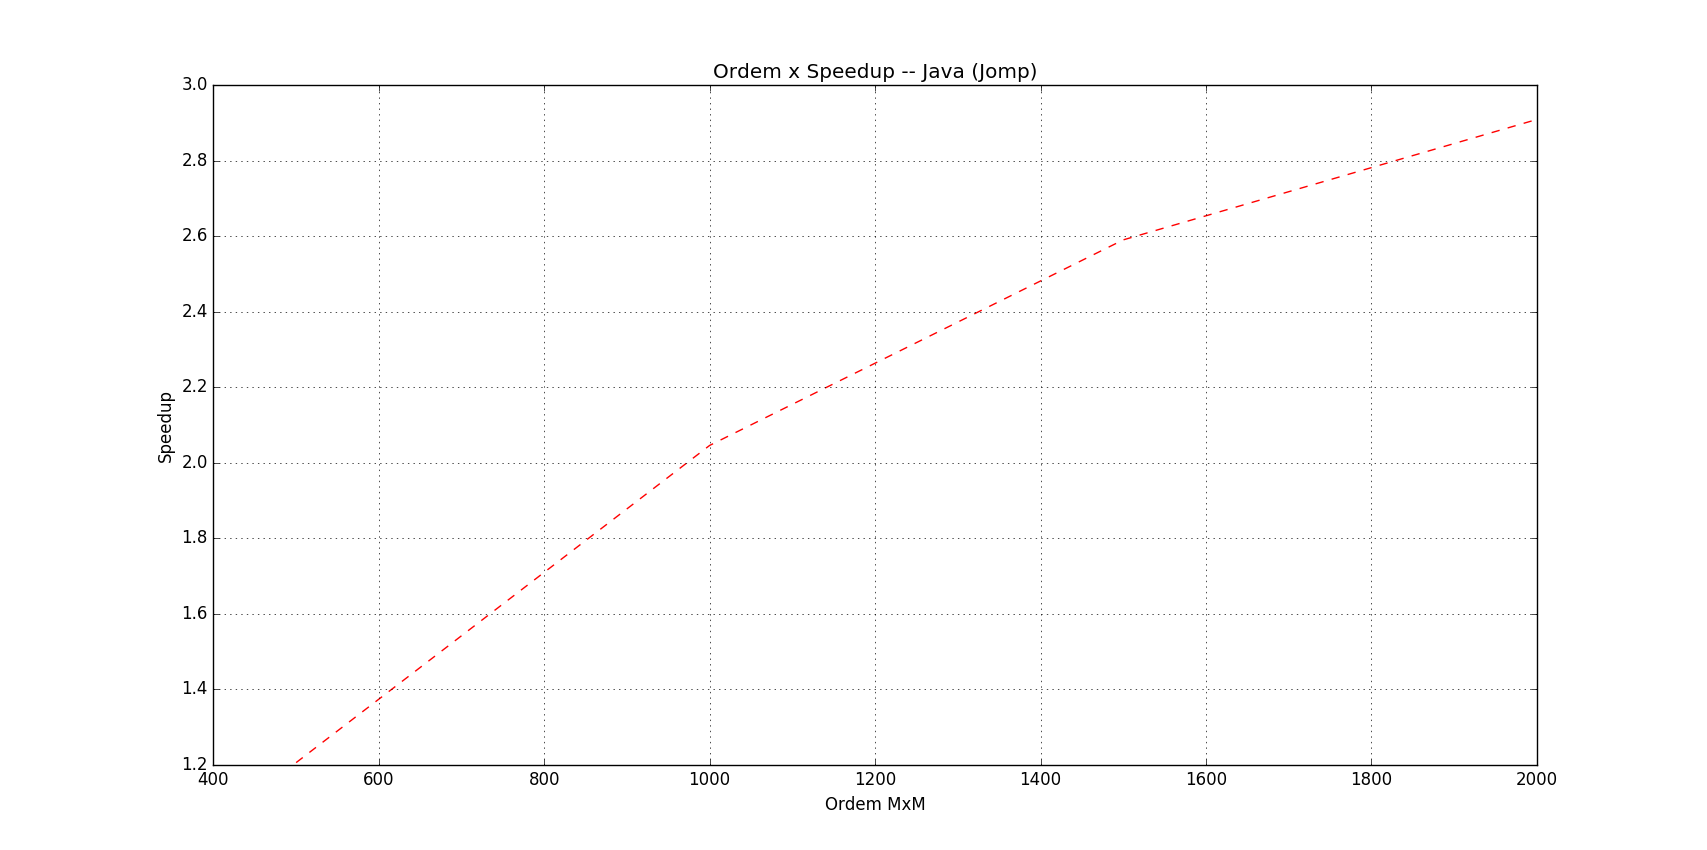
\includegraphics[width=15.0cm]{pictures/speedup_Java.png}
%  \caption{Ordem x Speedup - Java (Jomp)}
%\label{fig:speedup_Java}
%\end{figure}


\begin{table}[H]
  \centering
  \caption{Tempo de execução -- Cython}
  \begin{tabular}{ccc}
    \hline
    Matriz(ordem) & Serial(s) & Paralelo(s) -- Cython \\
    \hline
    \hline
    500 & 0.837 &  0.504 \\
    1000 & 10.186 & 3.841\\
    1500 & 30.911 & 12.314\\
    2000 & 1min41.794 & 29.442\\
    \hline
  \end{tabular}
  \label{tab:timePy1}
\end{table}


%\begin{figure}[!htb]  
%  \centering
%  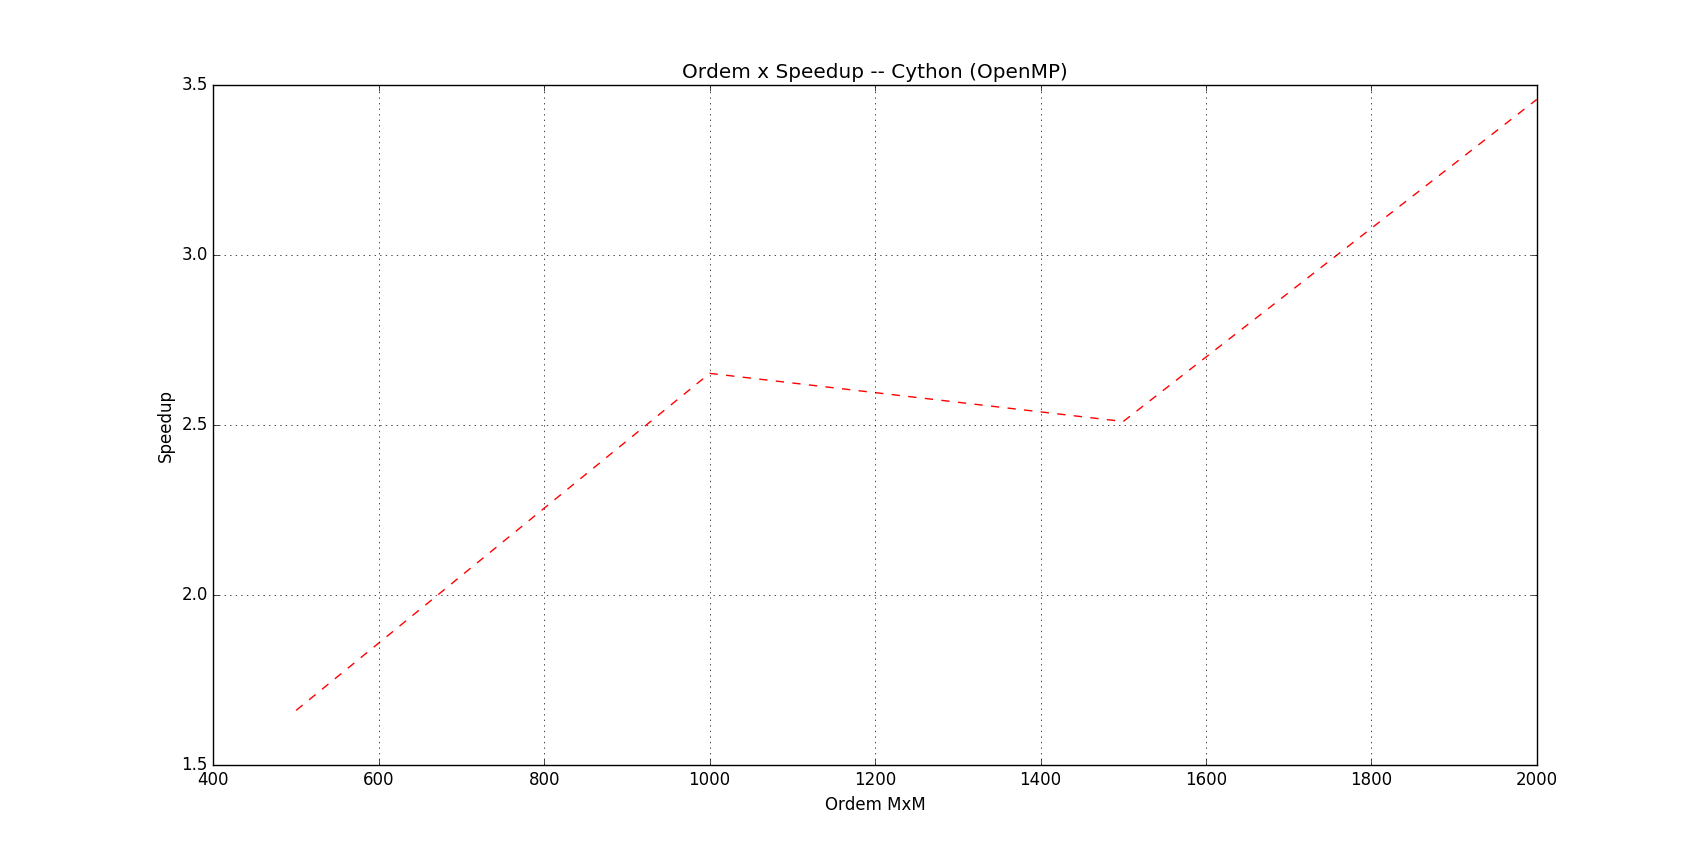
\includegraphics[width=15.0cm]{pictures/speedup_Cython.png}
%  \caption{Ordem x Speedup - Cython (OpenMP)}
%\label{fig:speedup_Cython}
%\end{figure}


Na execução do python com multiprocessing foi efetuada uma alteração no algoritmo serial. No lugar de uma multiplição entre matrizes, realizou-se duas multiplicações. Na prática, uma repetição foi inclusa na função de multiplicação. Dessa forma, tornou-se mais convincente o uso do paralelismo com multiprocessing, pois foi possível fazer com que cada processador executasse em paralelo uma multiplicação entre matrizes. Os tempos podem ser observados na tabela \ref{tab:timePy2}. 

\begin{table}[H]
  \centering
  \caption{Tempo de execução -- Python2.7}
  \begin{tabular}{ccc}
    \hline
    Matriz(ordem) & Serial(s) & Paralelo(s) -- Multiprocessing \\
    \hline
    \hline
    500 & 1.021 &  0.912 \\
    1000 & 17.073 & 9.797\\
    1500 & 1min7.847 & 31.116\\
    2000 & 2min27.214 & 1min17.700\\
    \hline
  \end{tabular}
  \label{tab:timePy2}
\end{table}


%\begin{figure}[H]
%  \centering
%  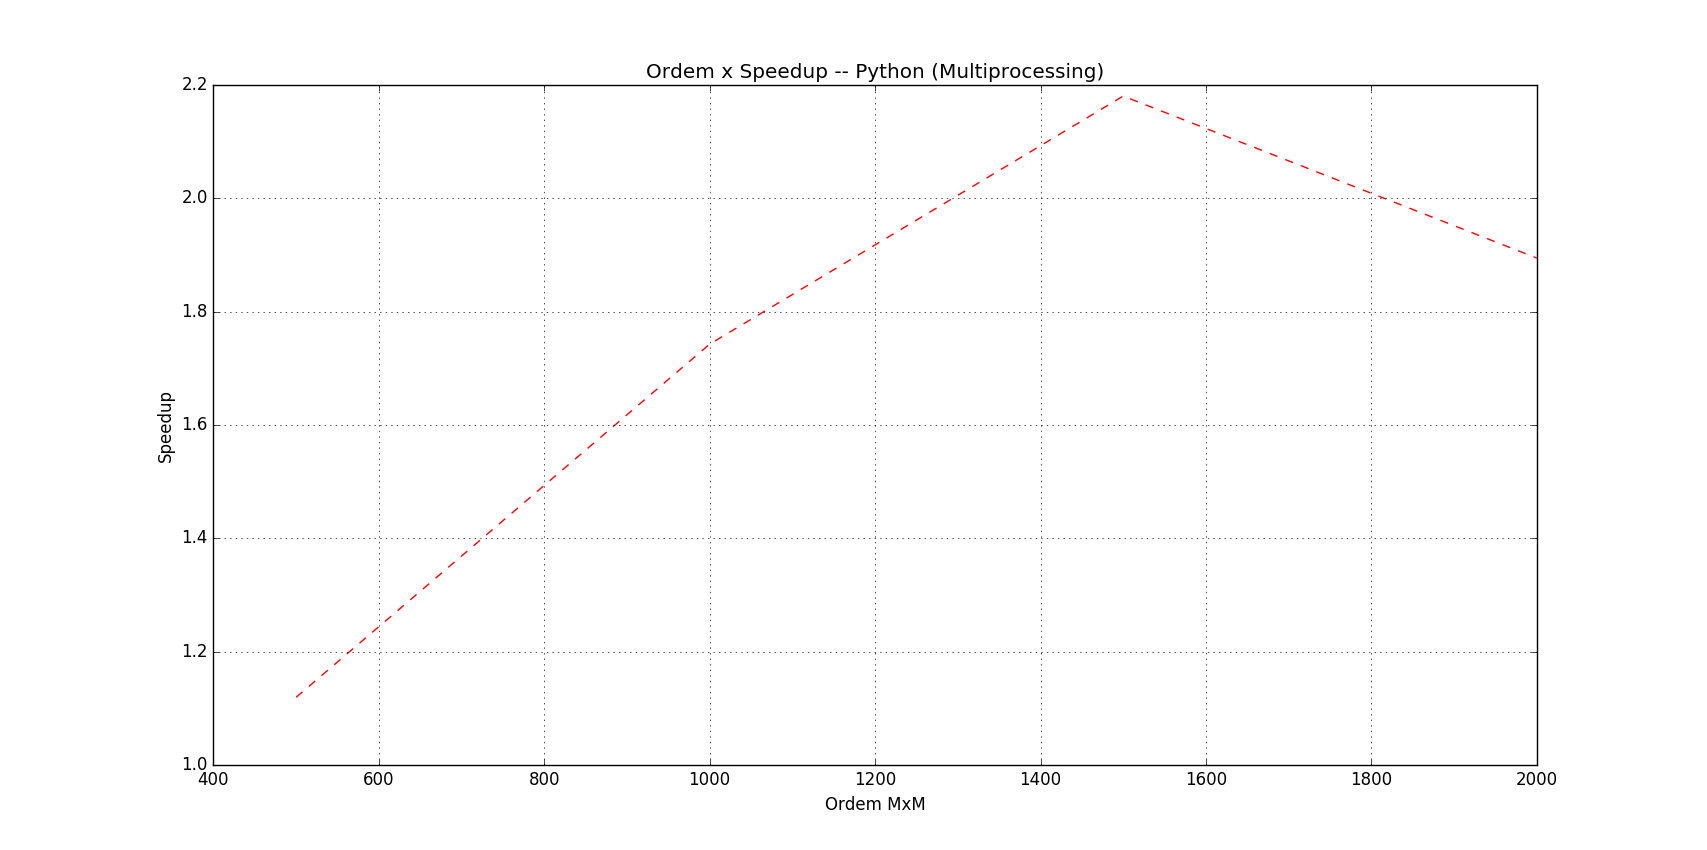
\includegraphics[width=15.0cm]{pictures/speedup_Python.png}
%  \caption{Ordem x Speedup - Python (Multiprocessing)}
%\label{fig:speedup_Python}
%\end{figure}

\begin{figure}[H]
  \centering
  \caption{Ordem x Speedup}
  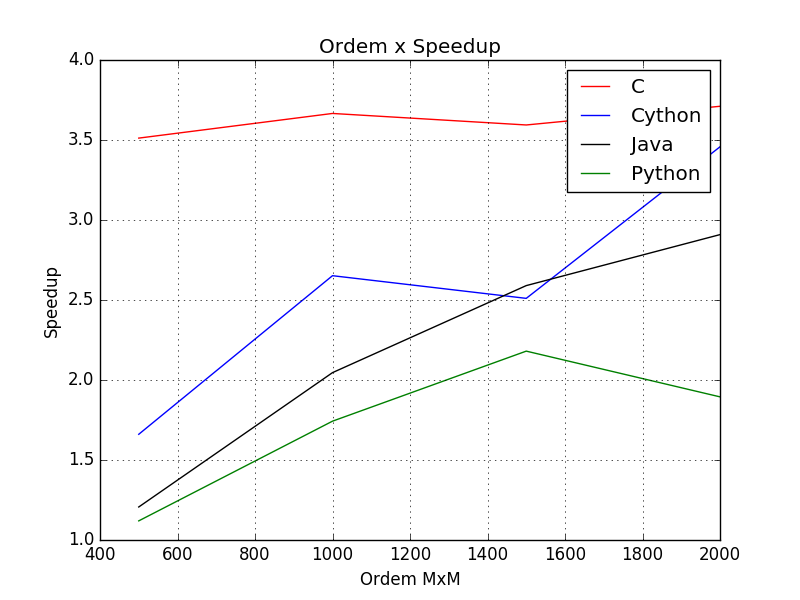
\includegraphics[width=11.0cm]{pictures/speedup_full2.png}\vfill
  \footnotesize{Fonte: Elaborada pelo autor.}
  
\label{fig:speedup_full}
\end{figure}


Conforme os valores obtidos e os gráficos gerados, é possível observar que a linguagem C obteve speedup entre 3.5 e 3.7, aproximadamente. O Python com multiprocessing obteve os menores valores de speedup, os quais variaram de 1 a 2, aproximadamente. Já o Cython e o Java ficaram entre 1 e 3, com uma leve vantagem para o Cython. A figura \ref{fig:speedup_full} ilustra o speedup de cada linguagem. 


\begin{figure}[H]
  \centering
  \caption{Tempo sequencial}
  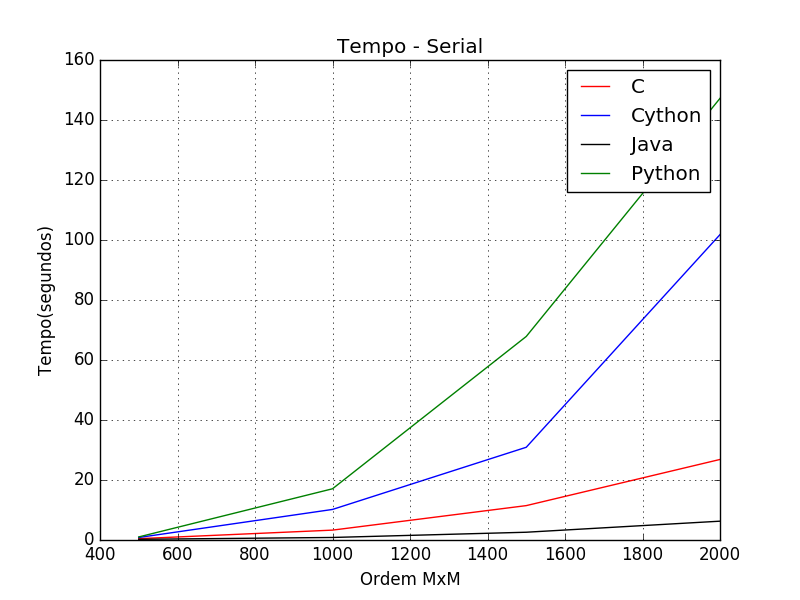
\includegraphics[width=11.0cm]{pictures/tempo_serial.png}\vfill
  \footnotesize{Fonte: Elaborada pelo autor.}
  
\label{fig:tempo_serial}
\end{figure}

\begin{figure}[H]
  \centering
  \caption{Tempo paralelo}
  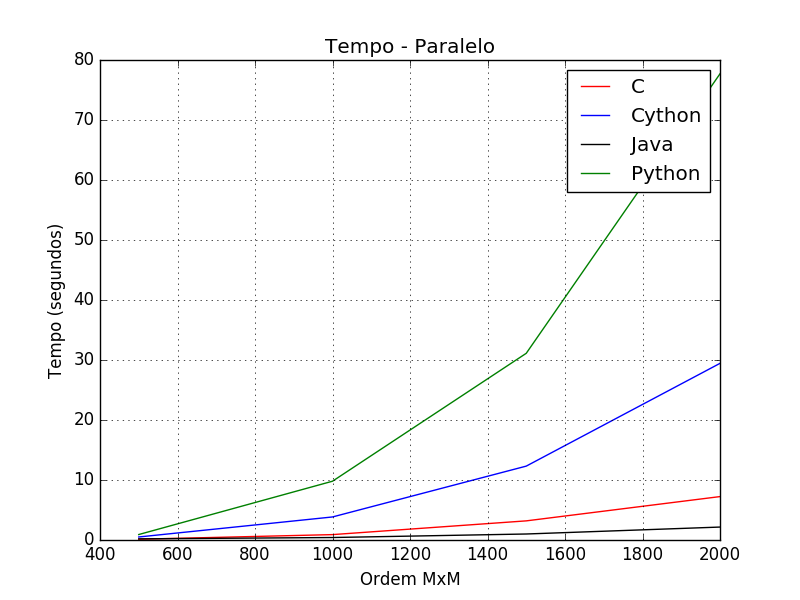
\includegraphics[width=11.0cm]{pictures/tempo_paralelo.png}\vfill
  \footnotesize{Fonte: Elaborada pelo autor.}
  
\label{fig:tempo_paralelo}
\end{figure}



\section{Considerações finais}
O trabalho comparou o desempenho de algoritmos seriais com paralelos. Os algoritmos implementaram uma multiplicação entre matrizes quadradas de ordem 500, 1000, 1500 e 2000. 

Em termos de tempo de execução, a linguagem Java foi a que obteve melhores resultados. Todavia, em termos de speedup, a linguagem C conseguiu atingir os valores mais altos. Lembrando, quanto maiores os valores, melhor desempenho aconteceu durante execução paralela. O speedup do Cython atingiu bons resultados e demonstrou que a linguagem cumpre as promessas de grande desempenho com relação ao Python. 

Exceto o Python com multiprocessing, as demais linguagens realizaram somente uma multiplicação entre matrizes. Isso aconteceu para que o módulo do multiprocessing fosse aproveitado de forma convincente, caso contrário não haveria ganhos. Por essa razão é possível notar um tempo serial de execução superior ao tempo serial da base de cálculo do Cython.

A partir dos resultados, que são bem limitados, nota-se que o emprego do OpenMP é mais vantajoso para a linguagem nativa, a saber, a C. Embora haja diversos projetos, bibliotecas ou módulos eficientes para as linguagens apresentadas nesse artigo, a interação entre API e linguagem ainda não é madura suficiente.  


\bibliographystyle{sbc}
\bibliography{references}


\end{document}
